\section{Proposed Method}
Existing specification-based malware detectors can be utilized if we extract
the correlation between shadow processes efficiently, because with that correlation
we are able to reconstruct the original system call graph from system call sequences
of shadow processes. In this section, we propose the design of a system method to extract the correlation.

\subsection{Problem Scope}
We focus on only shadow attacks that performs Inter-Process Communication, or IPC, via unix domain socket.

\cite{Weiqin:ShadowAttack} showed prototype implementation of a compiler
that takes existing malware as input and outputs the executable of malware of shadow-attack version.
Therefore, it is reasonable to infer that shadow attacks based on IPC through unix domain socket
are highly feasible, and they should be considered as a significant threat.

\subsection{Key Concepts (tentative)}
As mentioned before, shadow attacks are the strategy where malware exports its critical system calls
to shadow processes and hyde its malicious behavior.
\cite{Weiqin:ShadowAttack} listed examples of system calls that are critical for malware's intent,
shown in \Tref{tab:critical-system-calls}.

\begin{table*}[t]
  \caption{Examples of critical system calls. This table is reconstructed from \cite{Weiqin:ShadowAttack} by the author from.}
  \centering
  \begin{tabular}{|l|l|}
    \hline
    \textbf{Function Category} & \textbf{System Call}                     \\
    \hline
    File I/O operation         & open, read, write                        \\
    \hline
    Network                    & socket, connect, recv, send, read, write \\
    \hline
    Process management         & exec, execl                              \\
    \hline
  \end{tabular}
  \label{tab:critical-system-calls}
\end{table*}

Among these system calls, file-related and network-related system calls handle file descriptors:
\texttt{open} and \texttt{socket} create a new file descriptor,
while others access the file tied to the file descriptor or perform network communication.
So shadow processes need to transfer file descriptors to each other to perform the file-related and
network-related system calls. This concept is shown in \Fref{img:fd-transfer}.
To our best knowledge, file descriptor transfer through unix domain socket is a technology that, although not uncommon
in cloud-native environments \cite{Envoypro3:online,HAProxyT74:online},
is relatively rare in traditional Linux server environments
(that would be because the technology introduces unnecessary complexity and overhead in the system).
This situation makes the file descriptor transfer a unique characteristic of shadow attacks.

\begin{figure*}[t]
  \begin{center}
    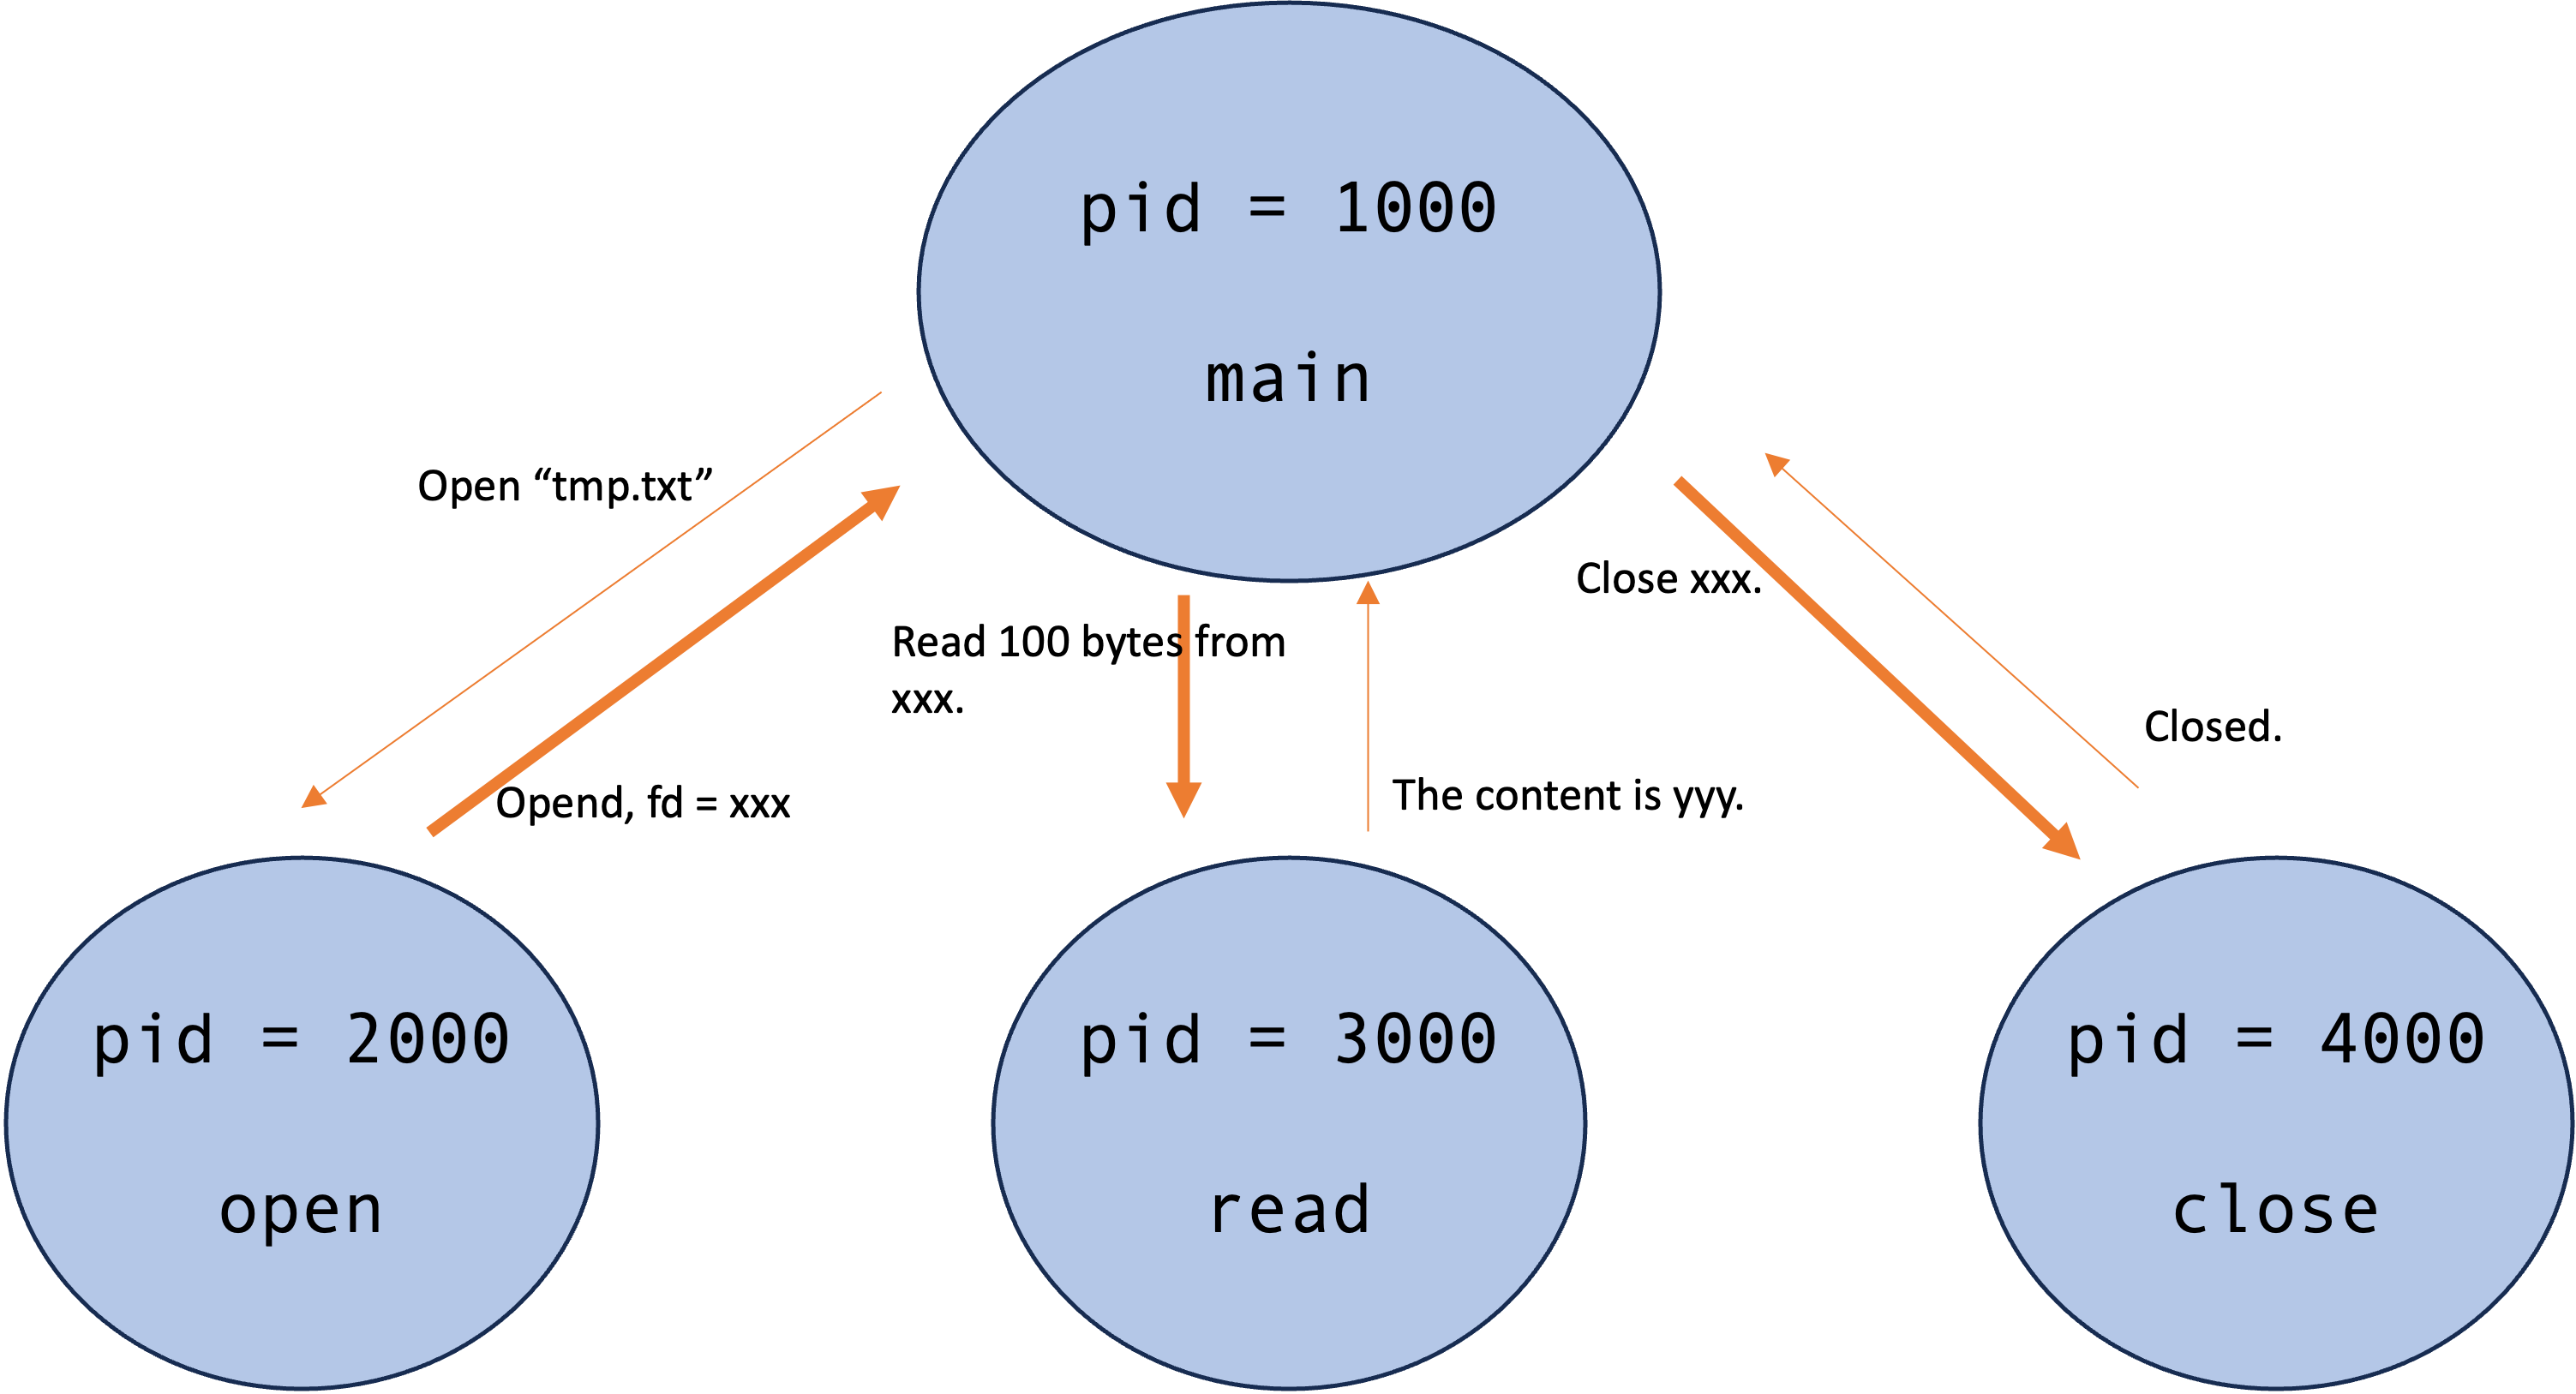
\includegraphics[width=1.8\columnwidth]{./img/fd_transfer.png}
  \end{center}
  \caption{Illustration of the concept of file descriptor transfer between shadow processes.
    The main process requests the shadow process to execute system calls, along with the required arguments.
    The thick arrows indicate the transfer of file descriptors over the control messages exchanged through IPC.}
  \label{img:fd-transfer}
\end{figure*}

\subsection{Design Overview}
